
\chapter{Einleitung}
\label{cha:Einleitung}
\dictum[Rainer Megerle (*1949), Chef Mergele AG, Nürnberg]{Es stimmt nicht, daß die Kosten die Preise bestimmen. Die im Markt erzielbaren Preise definieren die Kosten, die man sich leisten kann.}		
% -------------------------------------------------------------------------------------------------

\section{Motivation}

Das grundlegende Bestreben jedes Unternehmens ist es, seine Existenz am Markt zu sichern. Eine konjunkturell angespannte Wirtschaftslage, zunehmende Globalisierung der M\"arkte, h\"oherer Konkurrenzdruck und kontinuierlich steigende Anforderungen nach qualitativ hochwertigen Produkten stellen für die Unternehmen der Automobilindustrie wachsende Herausforderungen dar. 

Unsichere Absatzprognosen, ein erschwerter Zugang zu Kapital und ein stark erh\"ohter Preis- und Wettbewerbsdruck sind Probleme,
mit denen sich ein Automobilhersteller 2013 konfrontiert sieht. Dar\"uber hinaus erh\"ohen eine Vielzahl von international pr\"asenter Unternehmen den Konkurrenzdruck, den Bed\"urfnissen des Kunden gerecht zu werden.

Um diese Situation zu verbessern, geben die Automobilhersteller den Kostendruck an ihre Zulieferer weiter. So wirkt sich der Qualit\"ats - und Kostendruck und damit die Notwendigkeit, ein Bauteil schon w\"ahrend der Konstruktion fertigungsgerecht und somit kosteneffizient zu gestalten, direkt auf die Automobilzulieferer aus. Hieraus entsteht bei diesen Firmen die Nachfrage nach softwaretechnischen Werkzeugen, mit denen sich die Fertigungskosten eines Bauteils einfacher absch\"atzen lassen. 

\section{Problemstellung}

In der Automobilindustrie wird die Konstruktion s\"amtlicher Bauteile eines Fahrzeugs und ihr Zusammenbau zu Baugruppen mit Hilfe von Computer Aided Design-Systemen (CAD) realisiert. Dies hat unter anderem den Vorteil, das wichtige Untersuchungen bereits in einem fr\"uhen Stadium der Produktentwicklung durchgef\"uhrt werden k\"onnen. Das k\"onnen beispielsweise dynamische Simulationen des Fahrzeugverhaltens oder eben Kostenanalysen f\"ur Bauteile sein.

Zur Kostenanalyse von CAD-Bauteilen ist es notwendig, eine Reihe von Eigenschaften, die mit dem Fertigungsverfahren variieren, zu erfassen. Mit Fertigungsverfahren oder Fertigungsart sind eine Reihe von hintereinander ausgef\"uhrten Prozessen gemeint, mit denen ein Produkt aus anderen G\"utern produziert wird. Beispielsweise wird beim Spritzgie{\ss}en erhitzter Kunststoff in einen Hohlraum (Formwerkzeug) gespritzt, in welchem er erst verdichtet wird und dann erkaltet. Bei mit Spritzguss gefertigten Bauteilen sind Eigenschaften, die die Fertigungskostem ma{\ss}geblich erh\"ohen (sogenannte Kostentreiber) zum Beispiel die minimale und maximale Dicke des K\"orpers oder die Anzahl der sogenannten Hinterschnitte. Die Erfassung dieser Eigenschaften sind f\"ur den Benutzer teilweise sehr aufwendig, so das eine softwaretechnische Unterst\"utzung w\"unschenswert ist. Im Rahmen dieser Arbeit sollen Werkzeuge entwickelt werden, wie bestimmte kostentreibende geometrische Strukturen, sogenannte Rippen und Dome, innerhalb von spritzgego{\ss}enen Bauteilen einfacher ermittelt werden k\"onnen. Im folgenden Abschnitt \ref{injection} wird kurz auf die das Spritzgu{\ss} Fertigungsverfahren eingegangenen und die Anwendung GoCart vorgestellt, in die die im Rahmen dieser Arbeit entwickelten Werkzeuge integriert wurden.
 
\section{Kostenabsch\"atzung f\"ur spritzgussgefertigte Bauteile}
\label{injection}

Das Spritzgie{\ss}sen (oft umgangssprachlich auch als Spritzguss oder Spritzgussverfahren bezeichnet) ist ein sogenanntes Urformverfahren, das haupts\"achlich in der Kunststoffverarbeitung, aber auch beispielsweise beim Pulverspritzgie{\ss}en in der Metallverarbeitung eingesetzt wird.

Mit Hilfe dieses Verfahrens lassen sich direkt nutzbare Teile in gro{\ss}er St\"uckzahl herstellen. Dazu wir der jeweilige verfl\"ussigte  Werkstoff in Pulverform in eine Werkzeugform eingespritzt. Diese Werkzeugform definiert die Form und die Oberfl\"achenstruktur des zu fertigen Bauteils. Mit dem Spritzgu{\ss}verfahren lassen sich Bauteile mit sehr geringen Toleranzen, also sehr hoher Fertigungsgenauigkeit, in gro{\ss}en Mengen wirtschaftlich produzieren. 

Spritzgie{\ss}sen ist allerdings ein aufwendiger Fertigungsprozess, der nur bei hohen St\"uckzahlen wirtschaftlich ist. Hierbei machen die Kosten der Werkzeugh\"ullen ein gro{\ss}en Teil der Aufw\"ande aus. So ist die Rentabilit\"at von spritzgu{\ss}gefertigen Bauteilen erst bei einer St\"uckzahl von einigen tausend Teilen erreicht. Ma{\ss}geblich f\"ur die Kosten der Werkzeugh\"ullen sind unter anderem die Anzahl der Dom- und Rippenstrukturen des Bauteils. 

\subsection{Das Projekt GoCart}
\label{goCart}

Der praktische Teil der Masterarbeit wurd im Auftrag der Firma Teraport GmbH erstellt. Dieses Unternehmen besch\"aftigt sich mit der Entwicklung einer Reihe von modularen Softwarebausteinen (dem DMU-Toolkit), mit denen sich computergeometische Untersuchungen an triangulierten Fahrzeugdaten durchf\"uhren lassen. Dies sind zum Beispiel die Berechnung von Montagepfaden oder die \"Uberpr\"ufung von umfangreichen Geometrien auf Kollisionen. Die Werkzeuge der Teraport GmbH beinhalten auch die Visualisierungsanwendung, in die Komponenten

%Fertigungsgerechtes Konstruieren
%Spritzguss
%Kostentreiber bei Spritzguss

\subsubsection{Dome}
\label{dome}


\subsubsection{H\"andisches Ausmessen von Domstrukturen}
\label{domeMeasure}

Das h\"andische Messverfahren zur Platzierung eines parametrischen Zylinders erfordert zun\"achst die Eingabe einer beliebigen Anzahl von Punkten auf der planaren Oberfl\"ache der Domstruktur. Hierf\"ur wurde grafisches Werkzeug entwickelt, das es dem Benutzer erlaubt, eine Reihe von dreidimensionalen Kugelobjekten durch Linksklick im 3D-Ansichtsfenster zu erzeugen. Die Koordinate der jeweiligen Kugel wird bestimmt, indem der 3D-Selektionsmechanismus (eng. \textit{Picking}) der Anwendung genutzt wurde, um den Schnittpunkt eines Strahls vom Klickpunkt im Ansichtsfenster auf eine Objektgeometrie zu bestimmen.

Diese Kugeln m\"ussen vom Benutzer kreisf\"ormig auf der Zylinderkappe angeordnet werden. Durch Rechtsklick kann dann ein interaktiver parametrischer Messzylinder, mit dem H\"ohe und Radius manipuliert werden kann, erzeugt werden. Das Zylinderobjekt ist an der Normalen der sogenannten \textit{Best-Fitting Plane} ausgerichtet. Eine \textit{Best-Fitting Plane} f\"ur eine dreidimensionale Punktemenge ist diejenige Ebene, die den aufsummierten orthogonalen Abstand der Punkte zur Ebene minimiert. Sie wird sowohl f\"ur die halbautomatische Erkennung von Domstrukturen als auch f\"ur die Segmentierung der Bauteile, die in Abschnitt \ref{cha:segment} beschrieben wird, verwendet. Im Rahmen der Masterarbeit wurde das bestehende, auf Singulärwertzerlegung basierende Verfahren, durch Hauptkomponentenanalyse ersetzt. Es wird im Abschnitt \ref{subsec:pca} näher beschrieben.


Der Zylinder kann so im Schwerpunkt der Punktwolke und an der Normalen der Best-Fitting Plane ausgerichtet erzeugt werden. Als voreingestellter Radius wird der Abstand des am weitesten zum Schwerpunkt entfernten Punktabstand genutzt.
Der Benutzer kann dann mit Hilfe eines Transformationsmanipulators die Höhe und den Radius weiter anpassen.
%Beschreibung Dom
%Bild Dom

\subsubsection{Rippen}
Verst\"arkungsrippen sind ein wirksames Hilfsmittel, um die Steifigkeit und Festigkeit von Spritzgu{\ss}teilen zu erhöhen.
Der richtige Einsatz von Rippen kann Material und Gewicht einsparen, die Spritzzyklen verkürzen und dicke Querschnittbereiche vermeiden helfen, die beim Spritzgie{\ss}en zu Problemen führen könnten. Wenn Einfallstellen auf der einer Rippe
gegen\"uberliegenden Seite nicht akzeptabel sind, k\"onnen sie durch strukturierte Oberflächen oder andere geeignete Unterbrechungen im Bereich der Einfallstelle kaschiert werden.

%Bild Rippe


%Beschreibung GoCart
%Schmale
%Bild GUI
%Beschreibung Features



\begin{figure}[ht]
\centering
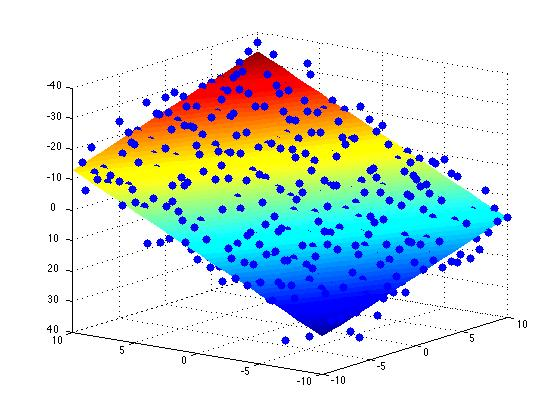
\includegraphics[width=10cm]{graphics/planefit.jpg}
\caption{H\"andische Erzeugung eines parametrischen Zylinders.}
\label{fig2}
\end{figure}



\subsubsection{H\"andisches Ausmessen von Rippenstrukturen}
\label{ribMeasure}

%Rippenmessen

\section{Grundlagen der verwendeten computergrafischen Techniken}

Dreidimensionale Objekte k\"onnen in einem Rechner nur visualisiert und verarbeitet werden, wenn ihre Struktur durch ein geeignetes Modell beschrieben wird. Ein einfaches solches Modell, auf denen die im GoCart-Projekt verarbeiteten Daten basieren, sind trinagulierte Geometrien. Sie werden im folgenden Abschnitt \ref{triGeo} n\"aher beschrieben.

In computergrafischen Systemen ist es oft erforderlich, den minimalen Abstand zwischen zwei geometrischen Objekten zu bestimmen. Um dies zu realisieren, sind effiziente Kollisionspr\"ufungsroutinen notwendig, auf die im Abschnitt \ref{colGeo} eingegangen wird.
 
In Abschnitt \ref{picking} werden kurz dreidimensionale Auswahlverfahren beschrieben.
 
\subsection{Triangulierte Geometrien}
\label{triGeo}

Eine einfache M\"oglichkeit zur Repr\"sentation von geometrischen K\"orpern sind Dreiecksnetze, sogenannte Triangulierungen. Eine Triangulierung approximiert die Oberfl\"ache eines K\"orpers durch (sehr kleine) Dreieckefl\"achen. Ein Dreieck ist ein planares Polygon und wird durch drei sogenannte Scheitelpunkte, oder eng. Vertices, definiert. Jeder dieser Scheitelpunkte beschreibt mittels x-,y- und z-Koordinaten eine Position im dreidimensionalen Raum. Triangulierungen sind ein Spezialfall polygonaler Flächenrepräsentation geometrischer K\"orper, die Objekte mit Hilfe von planaren Vielecken (Polygone) beschreiben. Das Verfahren funktioniert exakt f\"ur ebene Strukturen, bei gekrümmten Oberfl\"achen entsteht jedoch ein sogenannter Tesslierungsfehler, der umso stärker ausf\"allt, je weniger Dreiecke für die gekr\"ummte Oberfl\"ache verwendet werden. In Abbildung \ref{triangulation} ist dieses Verhalten deutlich zu erkennen: Die Triangulierung mit der h\"oheren Dreiecksanzahl wirkt an der Silhouette wesentlich runder als die mit geringerer Anzahl. 

\begin{figure}[H]
\centerline{
	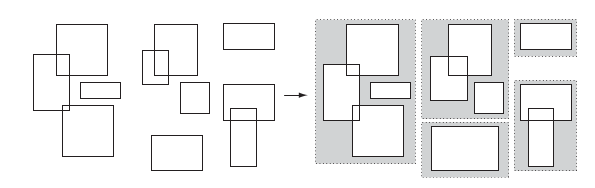
\includegraphics[width=0.7\columnwidth]{graphics/box.png}
}
\caption{Triangulierung eines Zylinders mit unterschiedlicher Dreiecksanzahl.}
\label{triangulation}
\end{figure}

Eine Triangulierung speichert neben den Punktdaten noch weitere Information f\"ur jedes Dreieck, wie beispielsweise Farbwerte oder sogenannte Normalenvektoren. Das sind Vektoren, die senkrecht auf der Netzoberfläche stehen und vom K\"orper  "`weg "` zeigen. Es wird zwischen Dreiecksnormalen und Punktnormalen unterschieden: Eine Dreiecksnormale ist der Vector, der orthogonal zur Dreicksfläche nach "`aussen"` zeigt. Die Punktnormale ist die Mittelung der  Dreiecksnormalen der drei Dreiecke, die an einen Scheitelpunkt angrenzen. Normalen haben in der Computergrafik verschiedenste Verwendungen, beispielsweise sind sie für essentiell f\"ur die Simulation von Oberfl\"achen in der Bildsynthese.

Eine Triangulierung kann gespeichert und maschinell verarbeitet werden, indem f\"ur jedes Dreieck die drei Scheitelpunkte explizit gespeichert werden. Dieses Verfahren ist allerdings \"ausserst unpraktisch, da zum einen Punkte mehrfach gespeichert werden und zum anderen keine M\"oglichkeit existiert, einfach benachbarte Dreiecke zu finden. Ein besseres Verfahren sind sogenannte indizierte Polygonmengen, eng. \textit{Indexed Face Set}. Hierbei werden alle Punkte in einer Liste gehalten. Ein einzelnes Dreieck kann dann durch drei Indizes in diese Liste beschrieben werden. Auf diese Weise ist zwar keine redundante Speicherung von Punktdaten mehr n\"otig, das Problem der fehlenden Nachbarschaftsbeziehungen besteht auch bei dieser Repr\"asentation. 

Dieses Problem wird beispielsweise mit der sogenannten \textit{Winged-Edge} Datesstruktur gel\"ost, die die gesamte Topologie durch Ecken beschreibt, die Referenzen auf benachbarte Fl\"achen und Scheitelpunkte beinhaltet. 

CAD-Fahrzeugmodelle liegen liegen zunächst in triangulierter Form vor. Diese kann mit Hilfe sogenannter Triangulierungungsverfahren aus der parametrischen Repr\"asentation (z.b. Nurbs oder Bezier-Patches), mit der innerhalb von CAD-Systemen gearbeitet wird, erzeugt werden. Die Algorithmen zur Triangulierung k\"onnen unter Umst\"anden fehlerhaft triangulierte Dreiecksnetze erzeugen. Oft auftretende Probleme sind beispielsweise Selbst\"uberschneidung von Dreiecken, kleine L\"ocher, doppelte Scheitelpunkte oder sogenannte T-Scheitelpunkte. T-Scheitelpunkte sind Scheitelpunkte, die auf einer Dreieckskante liegen (siehe Abbildung \ref{tvertice}). 

\begin{figure}[H]
\centerline{
	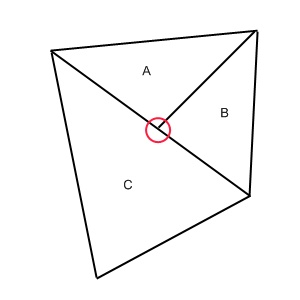
\includegraphics[width=0.4\columnwidth]{graphics/tvertices.jpg}
}
\caption{Triangulierung mit T-Scheitelpunkt.}
\label{tvertice}
\end{figure}

Einige Fehler wie doppelte Punkte oder kleine L\"ocher lassen sich durch verschiedene Bereinigungsverfahren beheben, andere, wie T-Scheitelpunkte, nicht.

\subsection{Kollisonspr\"ufung}
\label{colGeo}
 
 Unter Kollisionspr\"ufung versteht man im Allgemeinen das Erkennen von Ber\"uhrungen
oder \"Uberlappungen zweier oder mehrerer geometrischer Objekte im zwei- oder dreidimensionalen Raum.
Ein geometrisches Objekt ist hier ein K\"orper, der durch ein Polygonnetz oder
ein Freiformfl\"achenmodell beschrieben werden kann.

Es existieren eine Reihe weiterer Anwendungen, f\"ur die eine effiziente Kollisions\-pr\"ufung
unbedingt erforderlich ist:

\begin{itemize}
	\item Beim {\em Virtual Prototyping} wird die Baubarkeit der transformierten
	Einzelkomponenten des Prototyps durch Kollisionstests gew\"ahrleistet
    \cite{zachmannThesis}.
	\item In der {\em Pfad- und Bewegungsplanung} gilt es, f\"ur einen Roboter mit
	beliebigen Freiheitsgraden einen Weg von einem Start- zu einem Zielpunkt zu
	finden, ohne das dieser mit Hindernissen kollidiert \cite{lavalle}.
	\item {\em Starrk\"orper-Physiksimulationen}  f\"uhren Kollisionspr\"ufung aus,
	um in jedem Zeitschritt der Simulation zu erfassen, ob ein dynamisches Objekt mit einem
	anderen Objekt der Szene kollidiert. So k\"onnen nat\"urliche
	Verhaltensweisen starrer K\"orper, wie beispielsweise das voneinander Abprallen
	von Billardkugeln, simuliert werden.
\end{itemize}

Diese Anwendungen stellen unterschiedliche Anforderungen an ein
Kollisionspr\"ufungssystem. Zum einen m\"ussen in k\"urzerster Zeit \"Uberlappungen
zwischen dynamischen Objekten erkannt werden, zum anderen muss eine
gro"se Menge Geometrie verarbeitbar sein. Ein einfacher Ansatz, die Kollisionen
einer Szene zu finden, ist, alle Dreiecke paarweise gegeneinaner
zu testen. Dies f\"uhrt jedoch (bei  {\em n}
Szenenobjekten) zu quadratischem Aufwand:

\begin{equation}
\frac{n*(n-1)}{2} \in \mathcal O(n^2)\label{quad}
\end{equation}

So sind keine echtzeitf\"ahigen \"Uberlappungstests realisierbar! Daher muss die
Berechnungzeit mit Hilfe von Optimierungsmethoden minimiert werden. Eine Idee,
den Aufwand zu reduzieren, ist, einen Divide-and-Conquer Ansatz zu verwenden \cite{Ericson05}. 

%Sogenannte "`{\em Zwei-Phasen Algorithmen}"' wenden so einen Divide-and-Conquer Ansatz folgenderma"sen an:
%Zun\"achst wird in der "`{\em weiten Phase}"' (eng. "`{\em Broad Phase}") versucht, Paare von Objekten zu 
%finden, die miteinander kollidieren k\"onnten, weil sie r\"aumlich benachbart sind. Eine exakte  Kollisionserkennung %ist dann in der "`{\em nahen Phase}"' (eng. "`{\em Narrow Phase}") nur noch zwischen diesen Objekten erforderlich.

\begin{figure}[H]
\centerline{
	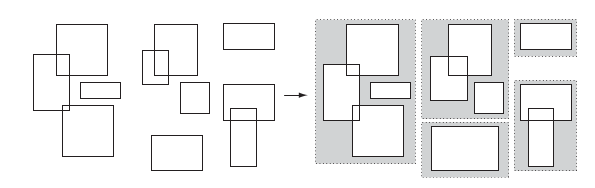
\includegraphics[width=0.7\columnwidth]{graphics/box.png}
}
\caption{Erkennung von disjunkten Objekten.}
\label{broadbox}
\end{figure}

In Abb. \ref{broadbox} sind auf der linken Seite um 11 Rechtecke auf Kollision zu pr\"ufen 55 Tests notwendig.
Nachdem in der "`weiten Phase"' 5 disjunkte Teilmengen erkannt wurden, kann die Anzahl der Tests in der "`nahen Phase"' auf 10 reduziert werden.

Ein Ansatz, die Anzahl der n\"otigen expliziten Dreiecks"-tests zu reduzieren, ist, anstelle der Dreiecke zun\"achst einen H\"ullk\"orper ({\em Bounding Volume}, kurz: {\em BV}) zu testen. Ein  H\"ullk\"orper ist ein
einfaches geometrisches Objekt wie beispielsweise ein W\"urfel oder eine Kugel, das das Objekt komplett
umh\"ullt. Die Idee ist, auszunutzen, dass die Schnitttests solcher K\"orper im Vergleich zu den eingeh\"ullten Objekten weniger aufwendig sind. So k\"onnen zun\"achst die Bounding Volumes zweier Objekte auf Kollision
getest\-et werden und nur dann, wenn dieser Schnitttest positiv verl\"auft, muss
die Dreiecksmenge der Objekte in der "`nahen Phase"' explizit gepr\"uft werden.

Die Nutzung von H\"ullk\"orpern reduziert den quadratischen Aufwand der Kollisionsp\"ufung einer Szene mit {\em n} Dreiecken soweit um einen konstanten Faktor {\em k}:
\begin{equation}
\forall k \in [0,1]:
k* \frac{n*(n-1)}{2} 
\in \mathcal O(n^2)
\end{equation}
Obwohl hierdurch der Rechenaufwand signifikant verringert werden kann, verbessert dies die Komplexit\"atsklasse des naiven Ansatzes nicht; die Anzahl der n\"otigen paarweisen Schnitttests zwischen den H\"ullen w\"achst noch immer
quadratisch bez\"uglich der Anzahl der Szenenobjekte.

Eine M\"oglichkeit, den Aufwand weiter zu reduzieren, ist die Nutzung von Hierachien aus H\"ullk\"orpern (sogenannten {\em Bounding Volume Hierachien} oder {\em BVH}). Dieser Ansatz wurde 1996 in dem Artikel "`{\em OBBTree: A Hierarchical Structure for Rapid Interference Detection}"' vorgestellt und hat seit dem die Forschung an Kollisionspr\"ufungsalgorithmen stark beeinflu"st \cite{Gottschalk}. BVH's betten die H\"ullk\"orper der Objekte rekursiv in gr\"o"sere BV's ein und ordnen diese in einer Baumstruktur an. So kann die Zeitkomplexit\"at des Algorithmus auf logarithmischen Aufwand verringert werden. Abbildung \ref{bvh} zeigt eine Hierachie weltachsenorientierter H\"ullquader, mit der f\"unf Objekte eingeh\"ullt werden.

\begin{figure}[H]
\centerline{
	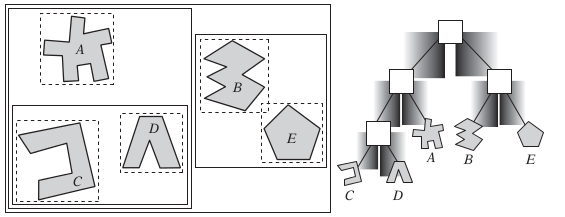
\includegraphics[scale=0.60]{graphics/bvh.png}
}
\caption{Bounding Volume Hierachie aus 5 Objekten. Auf der linken Seite wird
die Szene rekursiv umh\"ullt so dass die Baumstruktur auf der rechten Seite
daraus resultiert. }
\label{bvh}
\end{figure}

Der Ansatz rekursive H\"ullk\"orper in einer Baumstruktur anzuordnen, l\"asst
sich auch auf die Dreieckesmenge eines Objektes ausweiten. Hierbei wird die
Dreiecksmenge eines Objektes als Punktewolke interpretiert, die dann mittels
Top-Down Ans\"atzen so lange weiter unterteilt wird, bis ein Abbruchkriterium
erreicht ist. Abbildung \ref{bvho} zeigt eine solche Hierachie aus AABB's \"uber
der Dreiecksmenge eines Objektes.

\begin{figure}[H]
\centerline{
	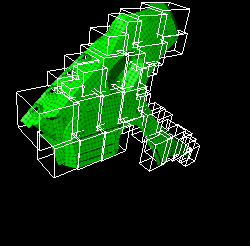
\includegraphics[scale=0.7]{graphics/BV-Hierarchie5.png}
}
\caption{Bounding Volume Hierachie \"uber den Dreiecken eines Objektes.}
\label{bvho}
\end{figure}

Um eine Szene, f\"ur die eine H\"ullk\"orperhierachie erzeugt wurde, auf Kollision zu testen, mu"s die Hierachie traversiert werden. Auf jeder Baumebene, die w\"ahrend der Traversierung besucht wird,  werden die BV's der Knoten
gegeneinander auf Kollision gepr\"uft. Wenn eine \"Uberschneidung zwischen zwei Bounding Volumes gefunden wurden, wird
die Baumsuche in diesen \"Asten fortgesetzt. Auf diese Weise wird rekursiv bis in die Blattknoten vorgegangen. Sollten die H\"ullen zweier Blattknoten \"uberlappen, kann eine Kollision zwischen den eingeh\"ullten Dreiecken bestehen, die dann in der "`Narrow Phase"' aufzul\"osen ist.

Im Rahmen dieser Arbeit wurde eine properit\"are Implementierung der frei verf\"ugbaren Bibliothek Proximity Query
Package (PQP) verwendet \cite{PQP}.

\subsection{3D-Selektion}
\label{picking}

Bei computergrafischen Anwendungen ist es oft notwendig, einen geometrischen K\"orper innerhalb einer Szene mit dem Mauszeiger zu selektieren. 

\begin{figure}[H]
\centerline{
	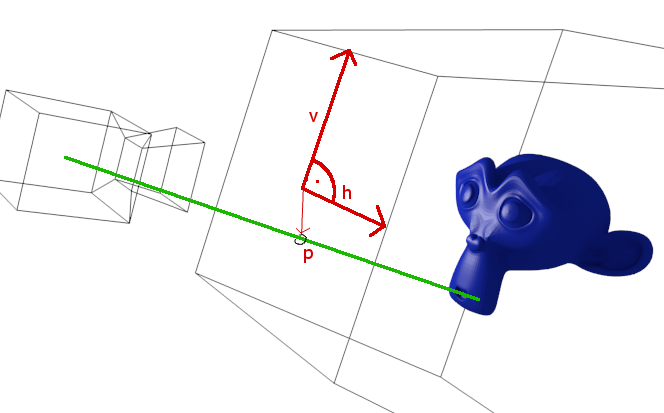
\includegraphics[scale=0.7]{graphics/raypicking.png}
}
\caption{Bounding Volume Hierachie \"uber den Dreiecken eines Objektes.}
\label{rayPicking}
\end{figure}

Eine typische Methode, dies umzusetzen, ist, einen Strahl vom Klickpunkt auf dem 3D-Ansichtsfenster der Anwendung \"uber die virtuelle Kamera in die Szene zu projizieren und zu testen,  ob der Strahl eine Geometrie schneidet (siehe Abbildung \ref{rayPicking}).
Dieses Verfahren wird als eng. \textit{Ray Casting} bezeichnet. Es hat den Vorteil, das es keine Methoden der zugrundeliegenden Grafikbibliothek benutzt und sich somit in jeder grafischen Anwendung auf die gleiche Weise verwenden l\"asst.

Um zu vermeiden, Schnittests zwischen jedem Dreieck der Szene
und dem Teststrahl durchzuführen, werden bei der Selektion mittels Ray Casting die Objektgeometrien, \"ahnlich wie bei der Kollisonspr\"ufung, durch H\"ullk\"orper ersetzt.

\section{Zielsetzung der Arbeit}
\label{problem}

\section{Aufbau der Arbeit}

